\chapter{Evaluation}
\label{ch:eval}
In this chapter we are going to define our experimental protocol as well as present and discuss our evaluation results.
\section{Experimental Setup}
\label{sec:experimentalsetup}
% Datasets, Methods, HW
We performed two sets of experiments, one for determining the best set of hyperparemeters and one for evaluating the performance of our approach on large scale datasets derived from real-world \ac{RDF} datasets.

All experiments were carried out on a $64$-core $2.3$ GHz server running \emph{OpenJDK} 64-Bit Server $1.8.0\_151$ on \emph{Ubuntu} $16.04.3$ LTS. 
Each experiment was assigned $128$~GB RAM.


%\section{Datasets}
%\label{ssec:datasets}

\section{Incremental Hyperparameter Optimization}
In order to determine the best set of values for our hyperparameters \emph{offspring fraction} $\alpha=\frac{\mu}{\lambda}$, \emph{mutation probability} $\sigma$ and \emph{mutation rate} $\rho$, we incrementally performed a series of grid searches.

\autoref{eq:grid} displays the values we considered in our first grid search.

\begin{equation}
  \begin{aligned}
    \alpha & \in \{0.0, 0.2, 0.4, 0.6, 0.8, 1.0\} \\
    \sigma & \in \{0.1, 0.3, 0.5, 0.7, 0.9\} \\
    \rho & \in \{0.1, 0.3, 0.5, 0.7, 0.9\} \\
  \end{aligned}
  \label{eq:grid}
\end{equation}

We started by setting up a minimal learning problem as follows.
First, we constructed a very simple toy dataset consisting of a single \ac{SCBD}.
Afterwards, we manually defined a linear enrichment graph with only three enrichment operators, the authority conformation, predicate conformation and \ac{NER} enrichment operators.
We derived our training example by applying this linear enrichment graph to the toy dataset.\\

Note that we set up this problem in a way such that the particular order of these enrichment operators is of no importance.
That is, as long as all three are present and are configured in the same way, the linear enrichment graph containing them will evaluate to the same result.\\

We set the number of rows in the enrichment tables to $r=7$, the population size to $p=30$ and the maximum number of generations to $g=5000$.\\

In order to have a good display of how efficient our approach can find perfect results, we disabled the convergence detection mechanism. 
We empirically found a seed $\texttt{seed}=54738$ for our \ac{PRNG} for which the initial population does not include a perfect genotype.\\

As our approach is non-deterministic, we needed to repeat the experiment a sufficient number of times.
This number was not obvious and therefore we empirically tried different orders of magnitudes $10^1, 10^2, 10^3$, where we repeated each series of repetitions ten times and measured the standard deviation of the average number of generations for each series of repetitions for all ten attempts.
When we set the repetitions to $10^3$, we could for the first time observe the standard deviation dropping to under $5\%$ of the mean number of generations.
We therefore sticked to this number of repetitions for all of the hyperparameter optimization experiments.\\

For this experiment we measured the mean, standard deviation, minimum and maximum of the generations until termination for each particular set of hyperparameters.

\begin{figure}[!tb]
\centering
\includestandalone[mode=image,page=1]{gfx/graphs}
\caption[First set of Hyperparameter Optimization Results]{\textbf{First set of Hyperparameter Optimization Results.} The experiment was repeated one thousand times. We measured the average as well as the standard deviation of the generations to termination. On the left hand side we see the average number of generations to termination plotted against the mutation probability $\sigma$ and the mutation rate $\rho$. The six planes correspond to the six values we tried for the offspring fraction $alpha$. We drew the best performing plane more opaque than the rest. On the right hand side we see a more detailed heat map of the best performing plane on the left. The results suggest that $\alpha=1.0$, $\sigma=0.9$ and $rho=0.9$ are the best performing hyperparameters for this experiment.}
\label{fig:eval1}  
\end{figure}

The results are shown in \autoref{fig:eval1}.
Note that the best set of hyperparameters we retrieved was $\alpha=1.0$, $\sigma=0.9$ and $\rho=0.9$.
The interpretation of those values is that for this particular experiment, the correct solutions are just found by chance, since this set of hyperparameters effectively maximizes the systems entropy.

This interpretation is further underlined by the high values we retrieved for the standard deviation of generations to termination, which can be seen as the coloring of the first plot in \autoref{fig:eval1}.

Despite these results are anything but surprising, as completely random manipulation of enrichment graphs can only lead to completely random results, they serve a good baseline to measure the success of the subsequential refinements of our baseline algorithm.\\

We continued to study the set of best hyperparameters for the same setting, but this time with the addition of the genotype compaction as described in \autoref{ssec:compaction}.

\begin{figure}[!tb]
\centering
\includestandalone[mode=image,page=2]{gfx/graphs}
\caption[Second set of Hyperparameter Optimization Results]{\textbf{Second set of Hyperparameter Optimization Results.} The experiment was repeated one thousand times. We measured the average as well as the standard deviation of the generations to termination. On the left hand side we see the average number of generations to termination plotted against the mutation probability $\sigma$ and the mutation rate $\rho$. The five planes correspond to the five values we tried for the offspring fraction $alpha$. We drew the best performing plane more opaque than the rest. On the right hand side we see a more detailed heat map of the best performing plane on the left. The results suggest that $\alpha=0.0$, $\sigma=0.1$ and $rho=0.1$ are the best performing hyperparameters for this experiment.}
\label{fig:eval2}  
\end{figure}

The results for this experiment are shown in \autoref{fig:eval2}.

Note that the first plot in \autoref{fig:eval2} is rotated by 180 degrees w.r.t. the first plot in \autoref{fig:eval1}.
Therefore, we get a completely different result this time, where the best set of hyperparameter amounts to $\alpha=0.0$, $\sigma=0.1$ and $\rho=0.1$.\\

However, despite these results looking very good, they are deceitful in that they are again just obtained by chance.
As we hoped for, the genotype compaction does indeed speed up the learning process by lowering the average number of generations needed to find a perfect genotype.
But since we always generate random rows to fill the genotype to its full capacity, we are actually just increasing the already considerable chance of finding a genotype that contains our set of enrichment operators in any order.\\

We therefore continued our investigation by increasing the hardness of the learning problem.
This time, we constructed two toy datsets as source training datsets.
Furthermore, we specified an inherently confluent enrichment graph that consisted of five enrichment operators.
This enrichment graph was developed in a way such that the enrichment operators did now depend on each other, so that it did not suffice to find an arbitrary permutation of them.\\

Note that with two dataset emitters and five enrichment operators, in order to find the perfect solution, our approach would need to work with its full capacity.
We therefore set the number of rows in our genotypes to $r=8$ to give the approach just a bit ,,space to breathe''.\\

After constructing this much harder learning problem, we then continued our investigation.
At first we wanted to have a good understanding of how much harder the new problem actually is compared to the old one.
To that end, we executed $10^3$ repetitions for the optimal set of hyperparameters $\alpha=0.0$, $\sigma=0.1$ and $\rho=0.1$ found previously, where the average number of generations to termination amounted to $2.77$.
The result of this run was that with an average number of generations to termination of $73.80$ the new problem was indeed much harder than the old one. In an extreme case, the perfect result was only obtained after 2636 generations.\\

Since due to the long runtimes it would have not been feasible to run a grid search for this problem with the current setting, we decided to instead introduce another addition to our algorithm, namely our graph merging crossover operator.\\

We left the rest of the setting untouched and ran the experiment again with an result of $36.99$ generations to termination on average.
Despite this being a substantial improvement, it was still not enough to run a complete grid search within an acceptable time, so we continued by introducing our precondition broadcasting mutation operator.\\

The new result looked very promising with an average number of generations to termination of only $15.23$, but still the maximum number of generations until a perfect solution was found was $528$.\\
In-depth analysis using the Java debugger made it evident that our approach was often stuck in local optima for extended periods of time.

We therefore enabled our convergence detection mechanism before we ran the next grid search.
Note that with the convergence detection mechanism we no longer necessarily retreived a perfect solution in each run.
Therefore, we measured the number of times that we actually did find a perfect solution.
Furthermore, we restricted the grid search for $\sigma$ and $\rho$ to the values $0.1, 0.3$ and $0.5$, as the previous results suggested that in order to achieve convergence, we should not introduce too much mutation into our system.

\begin{figure}[!tb]
\centering
\includestandalone[mode=image,page=3]{gfx/graphs}
\caption[Third set of Hyperparameter Optimization Results]{\textbf{Third set of Hyperparameter Optimization Results.} The experiment was repeated one thousand times. We measured the average generations to termination and the number of perfect runs. On the left hand side we see the number of perfect runs plotted against the mutation probability $\sigma$ and the mutation rate $\rho$. The six planes correspond to the six values we tried for the offspring fraction $alpha$. We drew the best performing plane more opaque than the rest. On the right hand side we see a more detailed heat map of the best performing plane on the left. The results suggest that $\alpha=1.0$, $\sigma=0.5$ and $rho=0.5$ are the best performing hyperparameters for this experiment.}
\label{fig:eval3}  
\end{figure}

The final results, which are shown in \autoref{fig:eval3}, suggest that the best set of hyperparameters are $\alpha=1$, $\sigma=0.5$ and $\rho=0.5$.

\begin{figure}[!p]
\centering
\makebox[0.5\textwidth][c]{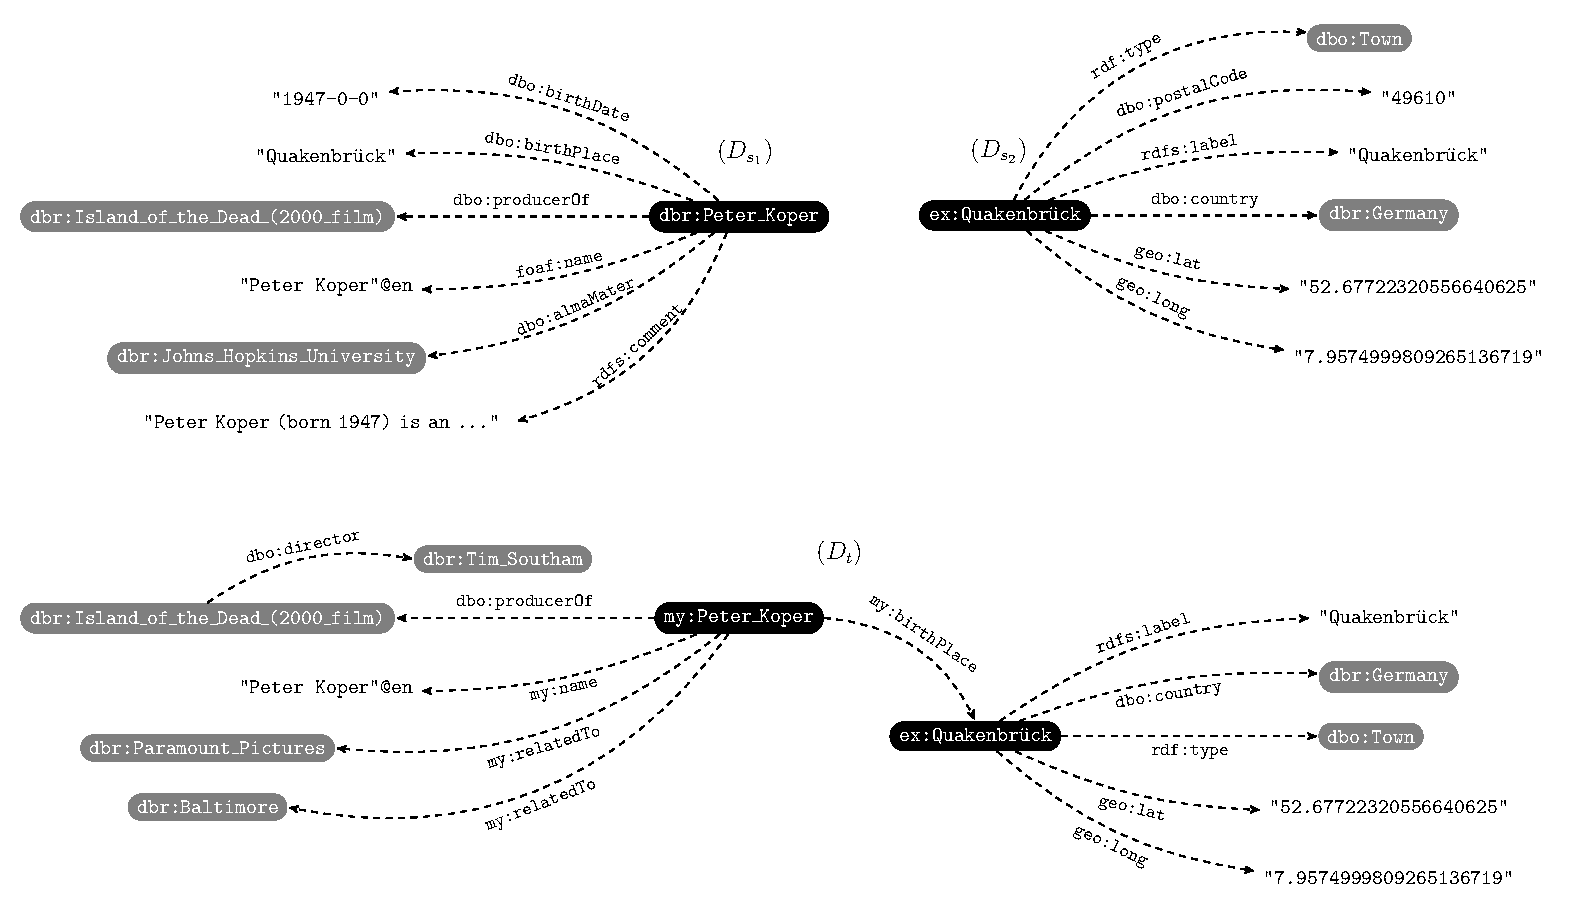
\includegraphics[width=1.25\textwidth]{gfx/img.pdf}}%
\caption[Performance Evaluation Setup]{\textbf{Performance Evaluation Setup.} (1) shows the \ac{SCBD} used as the first source training dataset. (2) shows the \ac{SCBD} used as the second source training dataset. (3) shows the target training dataset. (4) is the enrichment graph used to obtain (3) from (1) and (2). Within it, green nodes are dataset emitters, orange nodes are enrichment operators and the red node is the dataset acceptor. The letters in the orange nodes representing enrichment operators are the first letters of the corresponding enrichment operator, \ie \texttt{N} for the \ac{NER} operator, \texttt{A} for the authority conformation operator, \texttt{D} for the dereferencing operator, \texttt{L} for the linking operator, \texttt{P} for the predicate conformation operator and finally  \texttt{F} for the filter operator.}
\label{fig:performanceeval}  
\end{figure}

It is notable that for these hyperparameters we achieve $100\%$ perfect results despite enabling our convergence detection mechanism.
Another interpretation of the data worth of mentioning is that the average number of generations to termination is lower for other settings, but these settings did not achieve this amount of perfect results and the difference in run time is neglectable.

\section{Performance Evaluation}
\begin{figure}[!h]
\centering
\includestandalone[mode=image,page=4,width=0.6\textwidth]{gfx/graphs}
\caption[Performance Evaluation Results]{\textbf{Performance Evaluation Results.} We ran the performance evaluation experiment $50$ times with a maximum number of generation of $2,000$. The results suggest that the fitness generally grows rapidly over the first 20 generations. The generality of our results is underlined by the fact that the $95\%$-confidence intervals are always within $0.1$ of the measured average fitness over all repetitions.}
\label{fig:eval4}  
\end{figure}
This experiment was devised from real-world data coming from DBpedia\footnote{\url{https://dbpedia.org}}, where we obtained one dataset about $2,230$ persons born in Germany and another one about $1,660$ towns in Germany.

The source and target training datasets for this experiment are collectively shown in $\autoref{fig:performanceeval}$ together with the enrichment graph that was used to compute the target training dataset.

We measured the performance of our \acf{GP} algorithm by averaging the best fitness found in each generation over a series of fifty repetitions of this experiment.
Moreover, we measured run times of our algorithm.

In order to account for variance, we computed $95\%$-confidence intervals using Student's t-distribution.\\

The results in \autoref{fig:eval4} suggest that our approach will on average solve this task with an overall solution quality of over $99\%$ in under 500 generations.
Note that our approach took on average $16$ seconds to solve this problem with a minimum of $4$ seconds and a maximum of $30$ seconds.





% assure that research questions are answered
%\includestandalone
